\section{さまざまな「環境」}
\subsection{「環境」とは}
図表を挿入する際,\LaTeX では「環境(environment)」というものを宣言し,その中に図表を挿入する.環境は挿入するものによって分けられており,以下のように対応している.
\begin{description}
  \item[箇条書き]: itemize環境(順番をつけるときはenumerateなど)
  \item[数式]: align環境,equation環境など
  \item[図]: figure環境
  \item[表]: table環境
\end{description}
他にも様々な環境が存在するが,本誌では代表的な環境を紹介する.
また,環境を使用するときは基本的に\texttt{begin}コマンドではじめ,\texttt{end}コマンドで終了する.例えば,itemize環境を用いるときは以下のようになる.
\begin{itembox}[c]{環境の使い方}
  \texttt{
    \hspace{-0.5\zw}\textbackslash begin\{itemize\}\\
    \hspace{2\zw}\textbackslash item アイテムA\\
    \hspace{2\zw}\textbackslash item アイテムB\\
    \textbackslash end\{itemize\}
  }
\end{itembox}
\subsection{箇条書き}
通常の箇条書きにはitemizeを用いる.また,箇条書きする内容の先頭には\texttt{\textbackslash item}とつける必要がある.他にも箇条書きで用語を説明するdescriptionや,数字がつくenumerateも存在する.それぞれの例を以下に示していく.
\newpage
\subsubsection{itemizeの場合}
\begin{itembox}[c]{itemize環境を使う時のソースコード}
  \texttt{
    \hspace{-0.5\zw}\textbackslash begin\{itemize\}\\
    \hspace{2\zw}\textbackslash item アイテムA\\
    \hspace{2\zw}\textbackslash item アイテムB\\
    \textbackslash end\{itemize\}
  }
\end{itembox}
\begin{itemize}
  \item アイテムA
  \item アイテムB
\end{itemize}
\subsubsection{descriptionの場合}
\begin{itembox}[c]{description環境を使う時のソースコード}
  \texttt{
    \hspace{-0.5\zw}\textbackslash begin\{description\}\\
    \hspace{2\zw}\textbackslash item[説明A] アイテムA\\
    \hspace{2\zw}\textbackslash item[説明B] アイテムB\\
    \textbackslash end\{description\}
  }
\end{itembox}
\begin{description}
  \item[説明A] アイテムA
  \item[説明B] アイテムB
\end{description}
\subsubsection{enumerateの場合}
\begin{itembox}[c]{enumerate環境を使う時のソースコード}
  \texttt{
    \hspace{-0.5\zw}\textbackslash begin\{enumerate\}\\
    \hspace{2\zw}\textbackslash item アイテムA\\
    \hspace{2\zw}\textbackslash item アイテムB\\
    \textbackslash end\{enumerate\}
  }
\end{itembox}
\begin{enumerate}
  \item アイテムA
  \item アイテムB
\end{enumerate}
\subsection{数式}
一行で完結する数式,または複数行の数式に一つの式番号を振りたい場合は\texttt{equation}を,複数行の数式にそれぞれ連続した式番号を振りたい場合は\texttt{align}を用いる.なお,式番号を振りたくない場合は「*(アスタリスク)」をequationやalignの直後につける.
\subsubsection{equation}
\begin{itembox}[c]{equation}
  \texttt{
    \hspace{-0.5\zw}\textbackslash begin\{equation\}\\
    \hspace{2\zw}e\textasciicircum\{i\textbackslash pi\}=-1\\
    \textbackslash end\{equation\}\\
    \textbackslash begin\{equation\}\\
    \hspace{2\zw}\textbackslash begin\{split\}\\
    \hspace{4\zw}\textbackslash cos\textasciicircum2\textbackslash theta \& = \textbackslash cos\textasciicircum2\textbackslash theta -\textbackslash sin\textasciicircum2\textbackslash theta \textbackslash \textbackslash\\
    \hspace{4\zw}\& = 2\textbackslash cos\textasciicircum2\textbackslash theta - 1          \textbackslash \textbackslash\\
    \hspace{4\zw}\& = 1 - 2\textbackslash sin\textasciicircum2\textbackslash theta\\
    \hspace{2\zw}\textbackslash end\{split\}\\
    \textbackslash end\{equation\}
  }
\end{itembox}
\begin{equation}
  e^{i\pi}=-1
\end{equation}
\begin{equation}
  \begin{split}
    \cos 2\theta & = \cos^2\theta -\sin^2\theta \\
                 & = 2\cos^2\theta - 1          \\
                 & = 1 - 2\sin^2\theta
  \end{split}
\end{equation}
\subsubsection{align}
\begin{itembox}[c]{align}
  \texttt{
    \hspace{-0.5\zw}\textbackslash begin\{align\}\\
    \hspace{4\zw}\textbackslash cos\textasciicircum2\textbackslash theta \& = \textbackslash cos\textasciicircum2\textbackslash theta -\textbackslash sin\textasciicircum2\textbackslash theta \textbackslash \textbackslash\\
    \hspace{4\zw}\& = 2\textbackslash cos\textasciicircum2\textbackslash theta - 1          \textbackslash \textbackslash\\
    \hspace{4\zw}\& = 1 - 2\textbackslash sin\textasciicircum2\textbackslash theta\\
    \textbackslash end\{align\}
  }
\end{itembox}
\begin{align}
  \cos 2\theta & = \cos^2\theta -\sin^2\theta \\
               & = 2\cos^2\theta - 1          \\
               & = 1 - 2\sin^2\theta
\end{align}

\subsection{図}
図を挿入する際にはfigure環境を用いる.figure環境を用いることで,図にキャプションをつけることができる.また,図の位置を指定することもできる.
\begin{itembox}[c]{figure環境を使う時のソースコード}
  \texttt{
  \hspace{-0.5\zw}\textbackslash begin\{figure\}[htbp]\\
  \hspace{4\zw}\textbackslash centering\\
  \hspace{4\zw}\textbackslash includegraphics[width=12cm]\{sample.jpg\}\\
  \hspace{4\zw}\textbackslash caption\{画像サンプル\}\\
  \textbackslash end\{figure\}
  }
\end{itembox}
\begin{figure}[htbp]
  \centering
  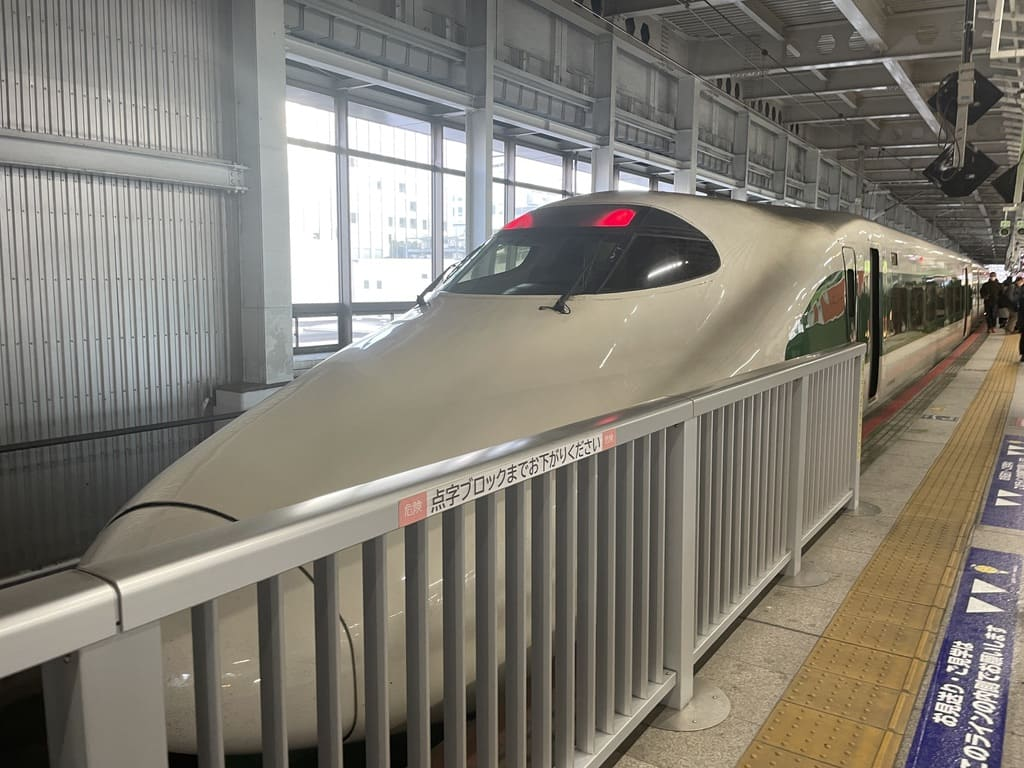
\includegraphics[width=12cm]{src/sample.jpg}
  \caption{画像サンプル}
\end{figure}
\subsection{表}
表を挿入する際にはtable環境を用いる.table環境を用いることで,表にキャプションをつけることができる.また,表の位置を指定することもできる.
\begin{itembox}[c]{table環境を使う時のソースコード}
  \texttt{
  \hspace{-0.5\zw}\textbackslash begin\{table\}[htbp]\\
  \hspace{4\zw}\textbackslash centering\\
  \hspace{4\zw}\textbackslash caption\{表サンプル\}\\
  \hspace{4\zw}\textbackslash begin\{tabular\}\{c|c\}\\
  \hspace{6\zw}\textbackslash hline タイトルA \& タイトルB \textbackslash\textbackslash\\
  \hspace{6\zw}\textbackslash hline 内容C \& 内容D \textbackslash\textbackslash\\
  \hspace{6\zw}\textbackslash hline 内容E \& 内容F \textbackslash\textbackslash\\
  \hspace{6\zw}\textbackslash hline\\
  \hspace{4\zw}\textbackslash end\{tabular\}\\
  \textbackslash end\{table\}
  }
\end{itembox}
\begin{table}[htbp]
  \centering
  \caption{表サンプル}
  \begin{tabular}{c|c}
    \hline
    タイトルA & タイトルB \\
    \hline
    内容C   & 内容D   \\
    \hline
    内容E   & 内容F   \\
    \hline
  \end{tabular}
\end{table}
\subsection{htbpとは}
図や表の位置を指定する際に,htbpというオプションを指定することがある.htbpはそれぞれ以下のような意味を持つ.
\begin{description}
  \item[h]: その場所に挿入
  \item[t]: ページの上部に挿入
  \item[b]: ページの下部に挿入
  \item[p]: 1ページにまとめて挿入
\end{description}
何も指定しない場合は,\LaTeX が自動で最適な位置に挿入する.しかし,ページ数が一番
少なくなるような位置に挿入するため,図や表が思った位置に挿入されないことが多い.
また,htbp指定でも必ずしも思った位置に挿入されるわけではない.どうしても図や表を
特定の位置に挿入したい場合は,hereパッケージを使って\texttt{[H]}オプションを
指定することで,その場所に図表を挿入できる.